\documentstyle[a4,isolatin1,times,ht01e, graphicx]{article}

\newcommand{\url}[1]{\textsf{#1}}
\newcommand{\hyp}{\discretionary{}{}{}}

\let\theirsection=\section
\renewcommand{\section}[1]{\theirsection{\MakeUppercase{#1}}}

\def\ra{$\rightarrow$}

\renewcommand\floatpagefraction{.9}
\renewcommand\topfraction{.9}
\renewcommand\bottomfraction{.9}
\renewcommand\textfraction{.1}   
\setcounter{totalnumber}{50}
\setcounter{topnumber}{50}
\setcounter{bottomnumber}{50}

\begin{document}

\def\figurewidth{\columnwidth}
\def\wfigurewidth{\textwidth}
\def\mockupwidth{16cm}

\title{The Internet RFCs as a hyperconnected document structure}

\authorname{Tuomas~J.\ Lukka, Rauli Ruohonen, Vesa Parkkinen, Antti-Juhani Kaijanaho
}
\authoraddr{  University of Jyv\"askyl\"a,
  Department of Mathematical Information Technology\\
  PO.~Box~35, FIN-40351~JYV\"ASKYL\"A, Finland\\
  E-Mail: \{lukka,raulir,veparkki,gaia\}@iki.fi
}
\maketitle

\begin{abstract}
  We propose the Internet RFC series as a corpus for testing new
  hypertext systems on.
\end{abstract}

\paragraph{KEYWORDS:} XXX

\section{Introduction}

It would be nice if there was a freely available nontrivial corpus that every

XXX Best would be if we could report on a successful application of RFCs...

\section{... some new stuff ...}

The Request for Comments (RFC)\cite{rfc-intro} series, published by
the Internet Society (``Network Working Group'' is listed on the
documents themselves as the publisher for historical reasons),
consists of over three thousand technical documents issued since 1969
and is currently growing at a rate of three hundred documents per
year.  An RFC is an ASCII text document that is never changed once
issued.  Most RFC documents are publically available on the Internet,
and only some historical documents originally distributed on paper are
missing from the electronic archives.

RFCs usually document or specify technical protocols, and sometimes
these specifications must be updated or replaced.  This is done by
issuing a new RFC document that is declared to obsolete or update some
other RFCs.  Currently about 500 RFCs are obsoleted by another RFC,
and and about 200 have been updated.  Since the RFC documents are
never modified, they only list those RFCs that they update or
obsolete; the reverse connection is not available in the RFCs.  This
problem is partly alleviated by \emph{The RFC Index}~\cite{rfc-index}
that lists every RFC, which RFCs they obsolete and update, and which
RFCs obsolete or update them.

An example of an RFC that is updated by many other RFCs is the
twenty-year-old Internet mail specification, RFC~822, which was
obsoleted in April 2001.  It was updated by five RFCs, including
RFC~1123, \emph{Requirements for Internet Hosts -- Application and
  Support}, which corrected and amended most standard protocols of the
time.  For an implementor of the mail protocol, it was imperative to
not just consider RFC~822 but also those updates of it that are
relevant for that implementor.

A problem of the RFCs is that the granularity of the update
relationships are 

It should be possible for a user of the RFC document series to see
updates at their proper positions:

The RFC series forms a corpus currently containing over a hundrded
megabytes of plain text.  


%\bibliographystyle{abbrv}
%\bibliography{gzigzag}
%\end{document}
\section{The Internet RFCs}

The RFC series forms a critical basis for the Internet standardization
effort: most technical standards which the Internet is based on have
been published in the last twenty years as RFCs (Requests For
Comments).  A history of the RFC series can be found
in~\cite{rfc-refguide} and in~\cite{thirty-years-of-rfc}.

% The RFC series, founded in 1969, was originally a series of
% working notes circulated among the early designers of the ARPANET,
% which later became the Internet.  Many of the earlier debates are
% still available in the RFC archives.  As the services of ARPANET grew
% and discussions could be held online via email and public discussion
% services, the RFC series became a publishing medium for results of
% those discussions.  

RFCs are divided into \emph{Standards Track}\/ RFCs and other
types, such as \emph{Informational}\cite{rfc-authoring,not-all-rfcs-are-standards}.  
A Standards Track
RFC is either an \emph{Internet Standard} or on its way to become
one\cite{ietf-standardization}.  
For example, the Internet email protocols and the Hypertext Transfer Protocol
(HTTP) are 
documented in Standards Track RFCs (see for example~\cite{rfc822}).
Most RFCs are also of a highly technical 
nature~\cite{rfc-intro}.  
%In essence, Standards Track RFCs document Internet's standard
%protocols in various stages of maturity~\cite{ietf-standardization}.

% Figure~\ref{fig-rfc-update} contains an example of an RFC that updates
% another RFC.

The actual RFC documents are rather long.  
For example, the RFCs used in the Figures of this article, 
1034, 2181 and 2308, which discuss the DNS (Domain Name System) 
are
17000, 5800 and 5900 words long, respectively --- and these three
are not the only ones concerning DNS.

The RFC series is considered to be an archival series:
once issued, an RFC is never modified~\cite{rfc-intro}.  Thus, when a
protocol documented in an RFC needs to be modified for whatever
reasons, a new RFC is issued.  Such an RFC either \emph{obsoletes} or 
\emph{updates} the RFC it is based on~\cite{rfc-authoring}.
If an RFC has been obsoleted, it is generally only interesting for
historical reasons. 
On the other hand, an RFC that has been updated retains its importance;
the updates usually only slightly change the content.
Among the abovementioned RFCs 1034, 2181 and 2303, the two latter
RFCs update the original 1034 by various amendments relating
to security, among other things.

%----------------------------------------------------------------------------
\section{Hypertextifying the RFCs}

Two hypertext versions of the set of all RFCs is available at
\cite{rfc-index-faqs} and \cite{armwar_rfc_hyper_archiv}.  
% Figure
% \ref{fig-example-current} shows the index entry of the first one and
% fragments of their version of RFC 1034.
The index entry shows which RFCs this RFC obsoletes as well as which
RFCs update it.  The text of the RFC itself has not been modified (see
below), and therefore the RFC itself only shows its relationship with
RFCs that came before it.

% Direct references to complete
% RFCs are shown as hyperlinks.

%\begin{figure}[htb!]
%\vbox{
%a) \\ 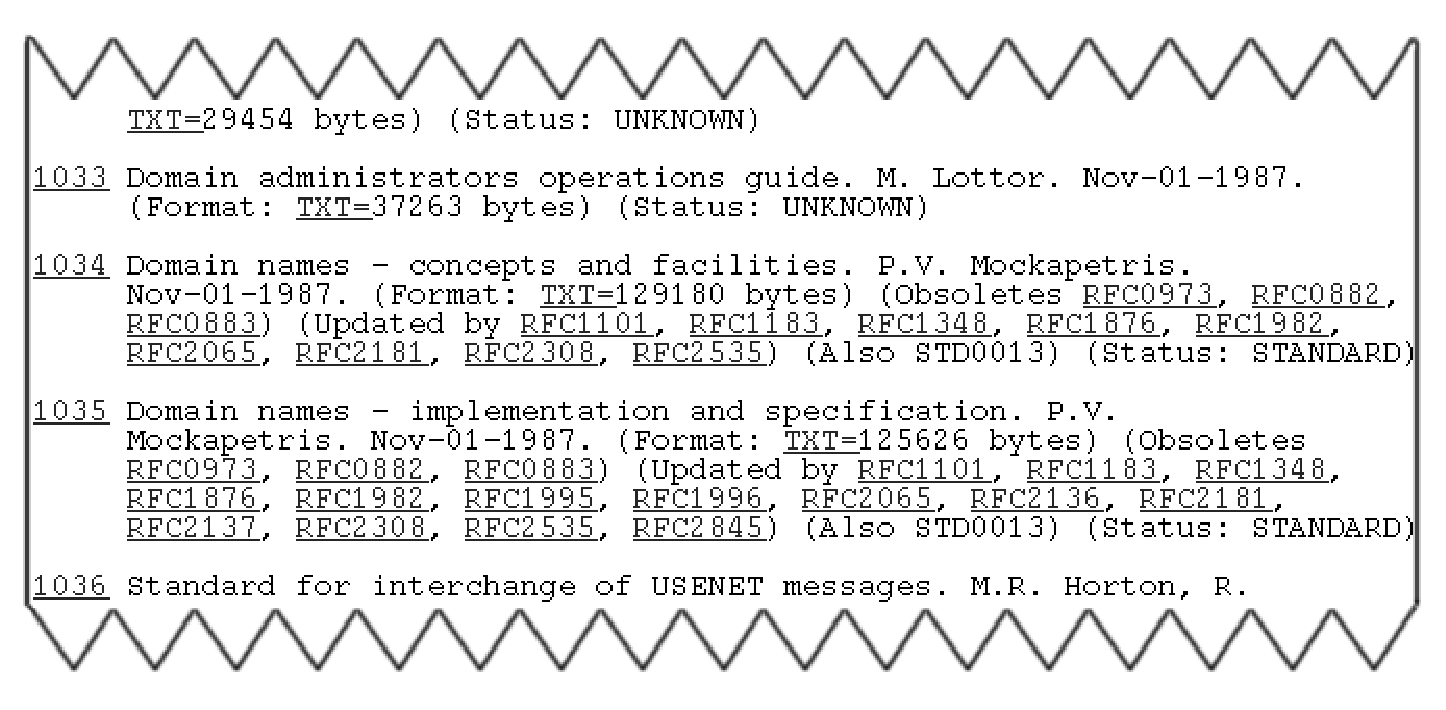
\includegraphics[width=\figurewidth]{HTML-RFC-index.ps} \\
%b) \\ 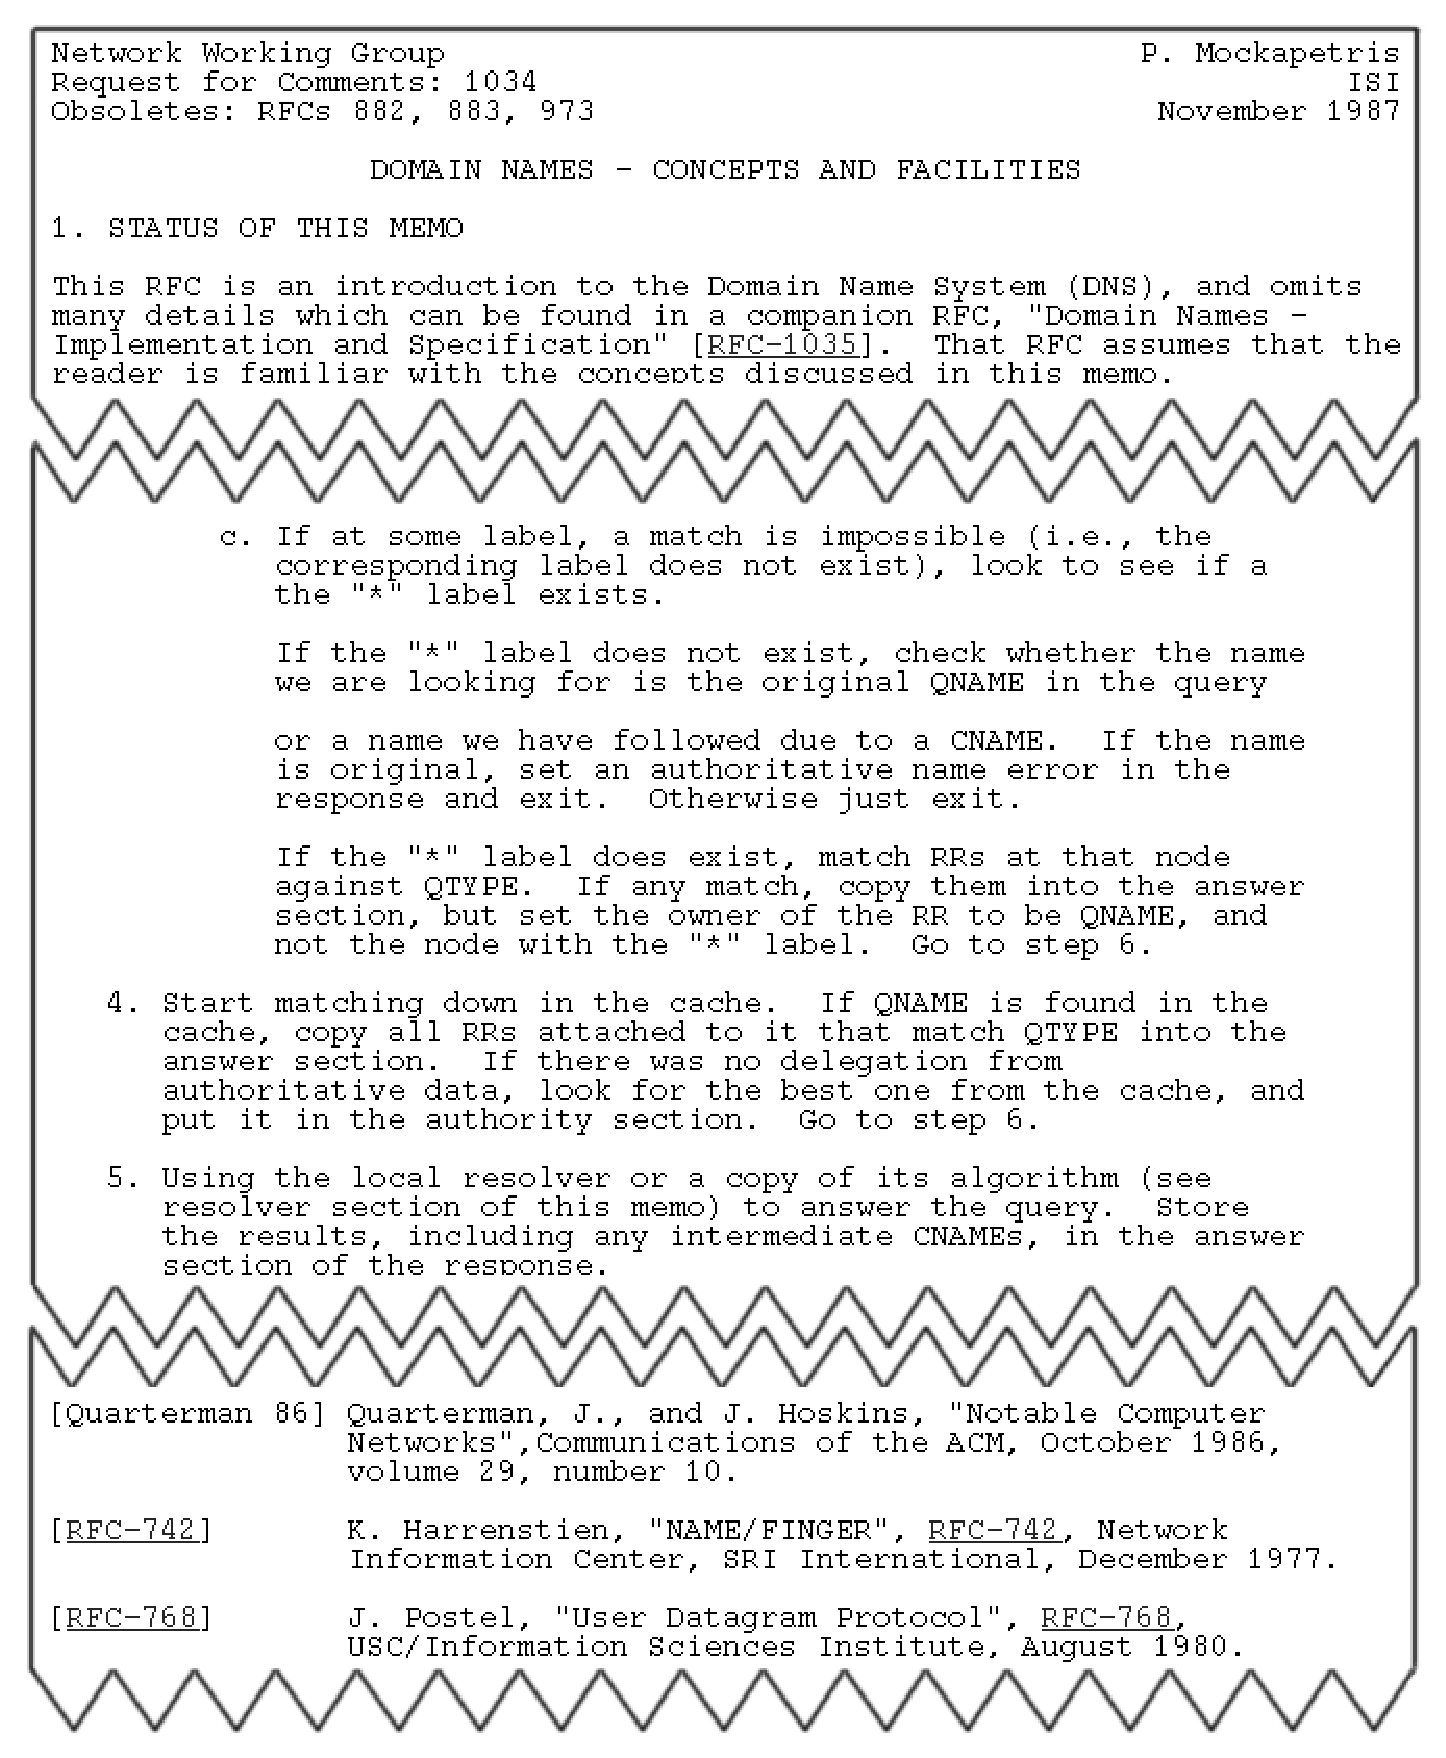
\includegraphics[width=\figurewidth]{HTML-RFC.ps}
%}
%\caption{a)The index entry at \cite{rfc-index-faqs} for RFC 1034
%b) Fragments of the hypertext version of RFC 1034 from \cite{rfc-index-faqs}.
%\label{fig-example-current}}
%\end{figure}

On the hypertext version of RFC 1034 from \cite{rfc-index-faqs}, no
reference is made to the RFCs that have later updated that RFC.  When
reading the the RFC, there is no way of knowing directly whether some
other RFC has updated the content of a given paragraph, since none of
the updated paragraph contain links to the updating RFCs.  This can be
a problem for the reader, since the longest and most important RFCs
naturally become the most heavily updated ones with time and the
updates can be of a crucial importance for e.g.~security or
interoperability.

It would therefore be an obvious
improvement to show links to sections that
update a given section. This cannot be done using normal in-line 
hyperlinks, as
issued RFCs may not be
modified~\cite{rfc-intro}, so
modifying a phrase to make a
smoothly worded inline hyperlink would be a copyright violation at
best~\cite{rfc-authoring}.  
One possibility is having an icon
(e.g.~``\emph{updated}'') as the link
source---this is not as
intrusive but the problem here is that a reader cannot know the nature
of the update, so following the link is essentially blind-folded
activity.  

One possibility, of course, is placing the links outside the text, in
the margin. This way, the text of the RFC remains untouched but
the link can state where it is going.
%Figure \ref{fig-updatelinks} shows how such a
%version could look. 
Creating a version such as this of all RFCs would be a monumental task
but would also save countless hours for later users.

% It is often tedious to try to find the right piece of information from RFCs
% due to their length and complexity. 
% Updates make the situation worse: even if the correct information is found,
% other RFCs have to be checked to see whether they change the XXX.

%\begin{figure*}[htb!]
%\centering
%\fbox{
%       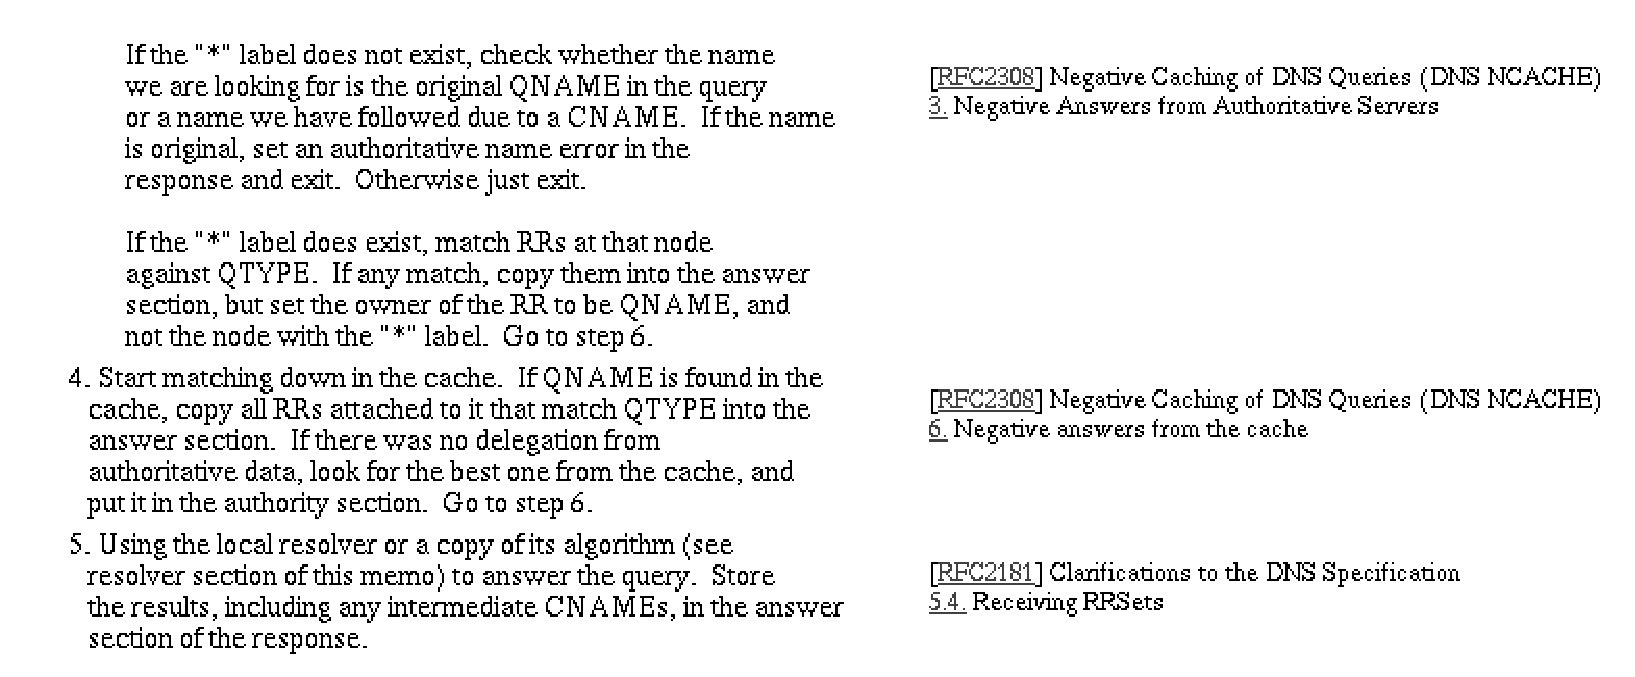
\includegraphics[width=\mockupwidth]{demo4.ps}
%}
%\caption{A HTML mock-up version of a fragment of RFC 1034,
%where the margin contains links to other RFCS that have been
%published later and contain updates relevant to these locations in 
%RFC 1034.
%\label{fig-updatelinks}}
%\end{figure*}

However, even here it is not immediately clear from the links what
the actual update in the updating RFC is. 
As Nielsen
states\cite{nielsen-links-as-microcontent},
links should be seen as microcontent, i.e.~an
ultra-short abstract of its target document. Thus, the users should
be made aware of what is at the other end of the link 
so that they can decide whether the linked-to document is
relevant to their current task.

The most unambiguous way is to simply display the complete
updating paragraph(s) from the updating RFC and vice versa.
%Figure \ref{fig-updatelarge} shows the same fragment of RFC 1034 as before
%in this type of display.
The problem with 
%the page in Fig.~\ref{fig-updatelarge} 
it is that the text of the
original RFC does not flow smoothly any more, since there is
too much updating information. 

Abstracting the nature of the update to fewer words is sometimes
possible but 1)~it would be an even more enormous task than simply
connecting the updating paragraphs for all currently used RFCs,
2)~the RFCs are already rather dense and it is not necessarily 
easy to find a good summary of the changes in a few words.

% Some of the above-mentioned problems can be solved by showing as much of the
% first updating paragraph as possible, with the constraints that the update
% must be centered to the updated paragraph and may not overlap with other
% updates. This is not much better, as it is less clear what is linked to what,
% and with cases such as the items 4.~and~5.\ of fig.~\ref{fig-updatelarge}
% there is no difference to the previously described clipping view.

In addition to showing the updates, 
it would also be desirable to show other
material related to the current paragraph from the same or other RFCs:
the RFCs contain a wealth of other intra- and intertextual structure
that would be useful for the reader to have at hand
in addition to the ``Updates'' relationship.

% such as a packet format or
% a command syntax.
% Readers not familiar with the subject
% would need definitions of terminology, and references to more obscure
% things such as the packet format is useful to any technical reader.
% Showing all this for every paragraph of the document is exteremly cumbersome,
% to say the least.


%\begin{figure*}[htb!]
%\centering
%\fbox{
%       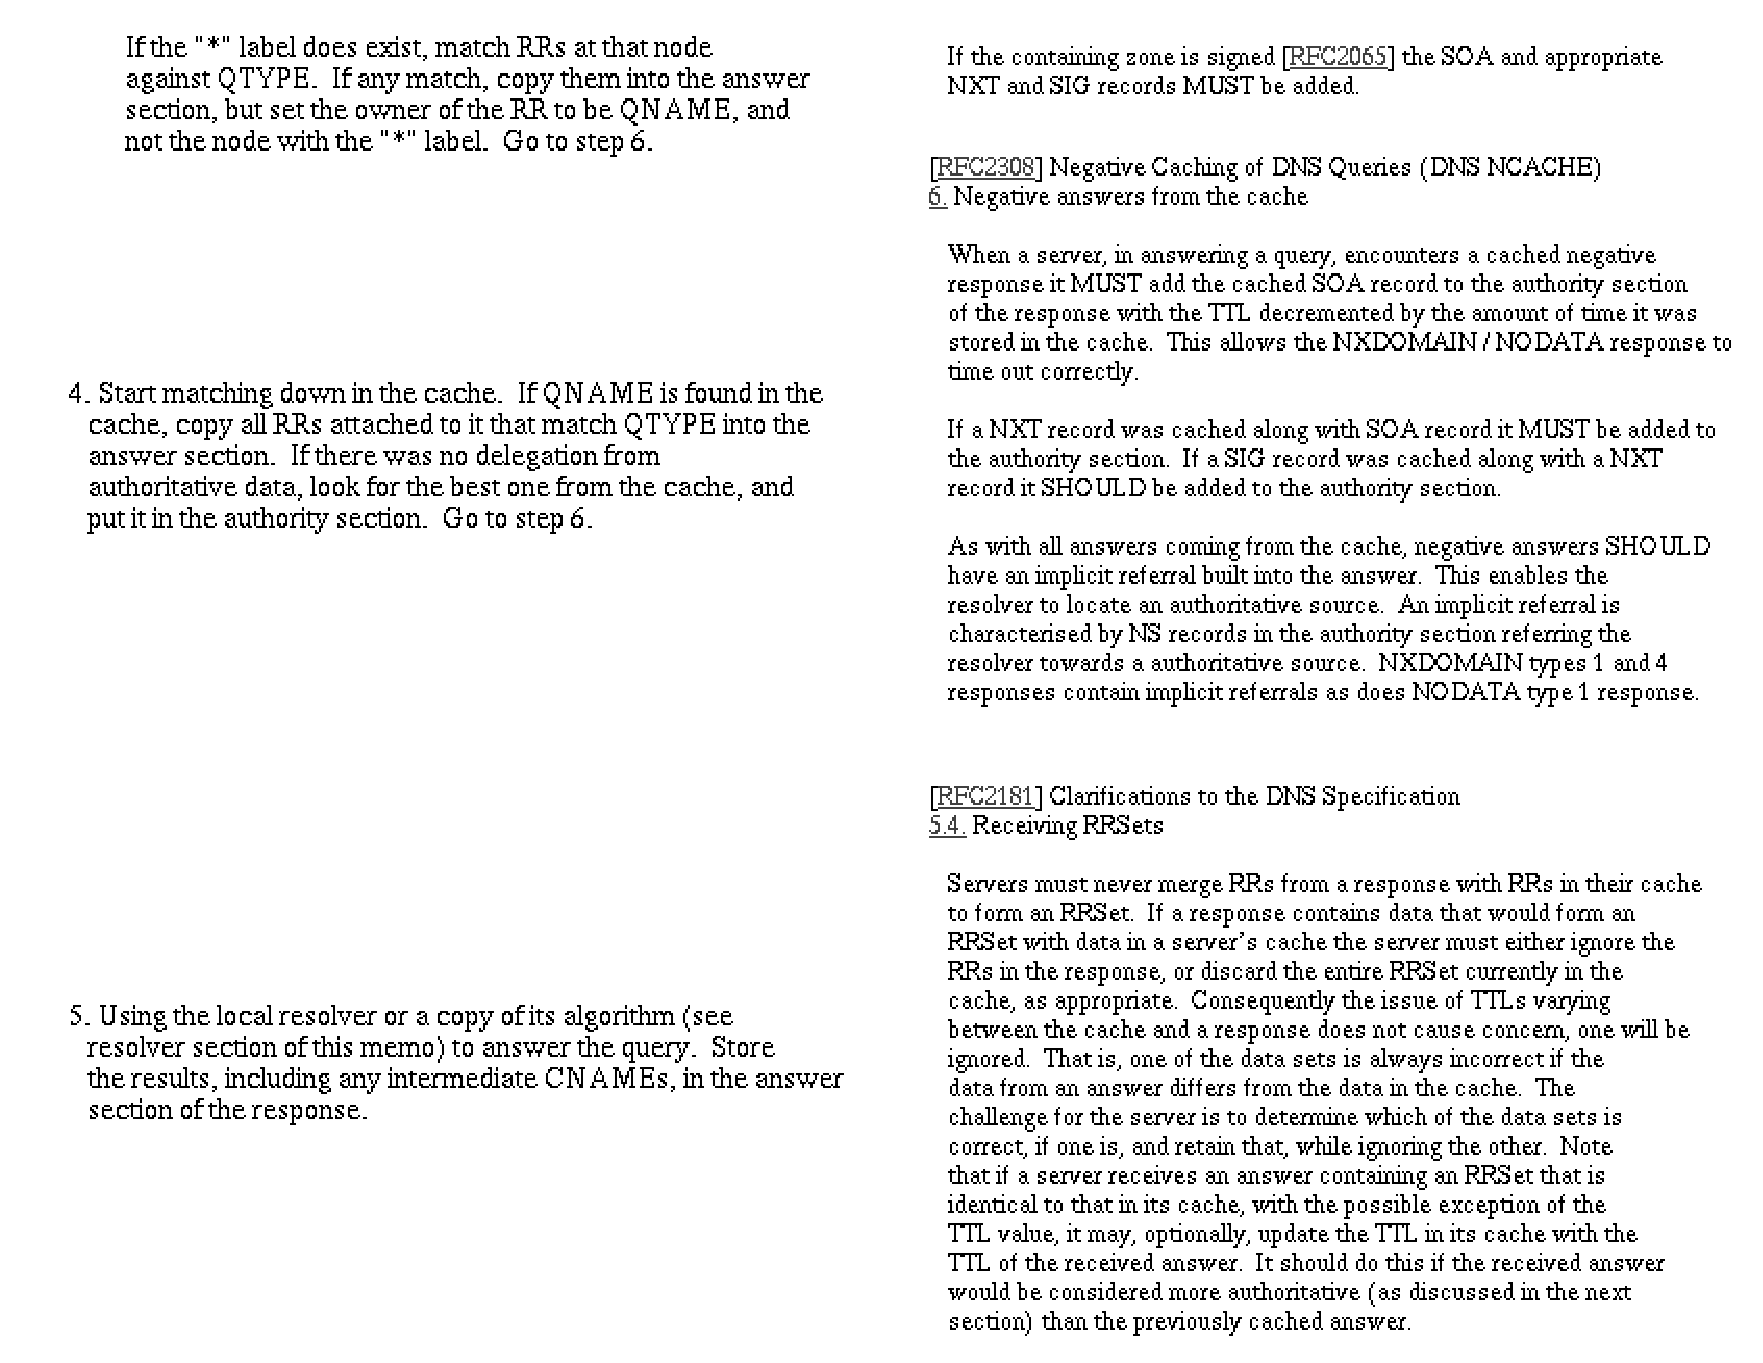
\includegraphics[width=\mockupwidth]{demo3.ps}
%}
%\caption{A mock-up HTML version of the same fragment as in Fig.~\ref{fig-updatelinks},
%where the actual paragraphs from the other RFCs that update this RFC
%have been included in the margin along with the links to give some more
%context for the links.
%The layout problems encountered by HTML are obvious.
%Additionally, the browser is unable to animate the text quoted from the other
%RFC to its new position on the screen when the reader follows the link to that 
%RFC --- the text will jump, causing disorientation for the reader.
%\label{fig-updatelarge}}
%\end{figure*}


\section{Conclusion}



\section{Acknowledgements}

The authors would like to thank Ted Nelson, Benjamin Fallenstein,
Kimmo Wideroos and Katariina Ervasti for interesting discussions.  The
authors gratefully acknowledge the stimulating comments from anonymous
reviewers of an earlier version of this paper.

\bibliographystyle{abbrv}
\bibliography{gzigzag}
 

\end{document}